\documentclass[10pt,a4paper,draft,twocolumn]{article}

\usepackage{amssymb}
\usepackage[english]{babel}
\usepackage{color}
\usepackage[colorlinks=false,%
            pdfkeywords={OCaml, Just In Time compilation, machine code generation},%
            pdftitle={Towards a usable native toplevel for OCaml},%
            pdfauthor={Marcell Fischbach, Benedikt Meurer},%
            pdfsubject={},%
            pdfdisplaydoctitle=true]{hyperref}
\usepackage{tikz}
\usepackage{varwidth}

\usetikzlibrary{arrows}
\usetikzlibrary{trees}
\usetikzlibrary{arrows,backgrounds,decorations.pathmorphing,fit,matrix,positioning}
\tikzset{
  phase/.style={
      rectangle,
      inner sep=1mm,
      rounded corners=1mm,
      minimum size=6mm,
      very thick,
      draw=blue!50!black!50,
      top color=white,
      bottom color=blue!50!black!20
  }
}

\begin{document}

\title{%
  Towards a usable native toplevel for OCaml
}
\author{%
  Marcell Fischbach\thanks{
    Universit\"at Siegen,
    D-57068 Siegen,
    Germany,
    \url{marcellfischbach@googlemail.com}
  }
  \and
  Benedikt Meurer\thanks{
    Compilerbau und Softwareanalyse,
    Naturwissenschaftl.-Technische Fakult\"at,
    Universit\"at Siegen,
    D-57068 Siegen,
    Germany,
    \url{meurer@informatik.uni-siegen.de}
  }
}
\date{}

\maketitle

\begin{abstract}
  TODO
\end{abstract}


%% Introduction
\section{Introduction}

The OCaml \cite{Leroy11,Remy02} system is the main implementation of the Caml
language \cite{Caml11}, featuring a powerful module system
combined with a full-fledged object-oriented layer. It comes with an optimizing native
code compiler \texttt{ocamlopt}, for high performance; a byte code compiler \texttt{ocamlc}
and interpreter \texttt{ocamlrun}, for increased portability; and an interactive top-level
\texttt{ocaml} based on the byte code runtime, for interactive use of OCaml through a
read-eval-print loop.

\texttt{ocamlc} and \texttt{ocaml} translate the source code into a sequence of byte code
instructions for the OCaml virtual machine \texttt{ocamlrun}, which is based on the ZINC
machine \cite{Leroy90} originally developed for Caml Light \cite{Leroy02}. The optimizing
native code compiler \texttt{ocamlopt} produces fast machine code for the supported targets
(at the time of this writing, these are Alpha, ARM, Itanum, Motorola 68k, MIPS, PA-RISC, PowerPC,
Sparc, and x86/x86-64), but is currently only applicable to \emph{static program compilation}.
For example, it cannot yet be used with multi-stage programming in MetaOCaml \cite{Taha03,Taha06},
the Coq proof assistant \cite{Bertot04,Coq10}, or the interactive toplevel \texttt{ocaml}.

This paper presents our work on a new native OCaml toplevel, called \texttt{ocamlnat}, which is
based on the native runtime and the compilation engine of the optimizing native code compiler.

TODO


%% Overview of the OCaml system
\section{Overview of the OCaml system} \label{section:Overview_of_the_OCaml_system}

This section gives a brief overview of the OCaml system. Additional details about the
byte code compiler and runtime can be found in \cite{Leroy90}, \cite{Meurer10ocamljit}
and \cite{Starynkevitch04}.
Feel free to skip to \textbf{TODO} if you are already familiar with the details.

\begin{figure}[htb]
  \centering
  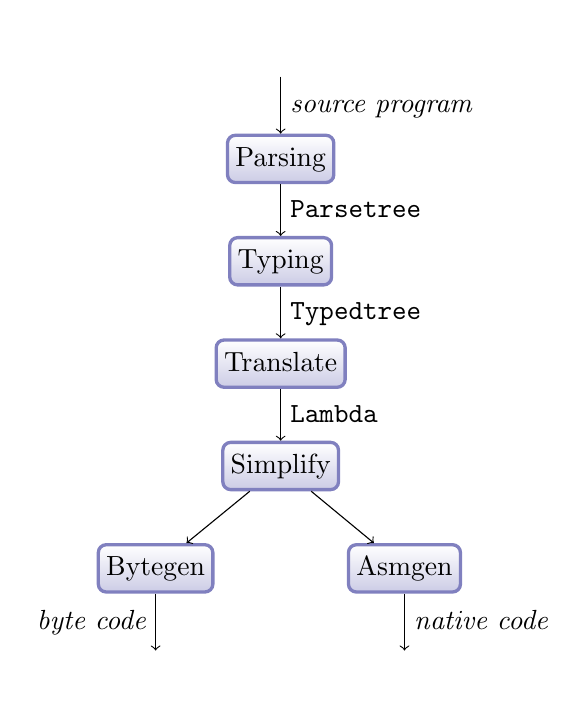
\begin{tikzpicture}[node distance=8mm,text height=1.5ex,text depth=.25ex]
    \matrix[row sep={1.3cm,between origins}]
    {
      & \node (start) {}; \\
      & \node[phase] (parsing) {Parsing}; \\
      & \node[phase] (typing) {Typing}; \\
      & \node[phase] (transl) {Translate}; \\
      & \node[phase] (simplif) {Simplify}; \\
      \node[phase] (bytegen) {Bytegen}; && \node[phase] (asmgen) {Asmgen}; \\
      \node (bytecode) {}; && \node (nativecode) {}; \\
    };
    \draw[->] (start) -- node[right] {\it source program} (parsing);
    \draw[->] (parsing) -- node[right] {\tt Parsetree} (typing);
    \draw[->] (typing) -- node[right] {\tt Typedtree} (transl);
    \draw[->] (transl) -- node[right] {\tt Lambda} (simplif);
    \draw[->] (simplif) -- node[left] {} (bytegen);
    \draw[->] (simplif) -- node[right] {} (asmgen);
    \draw[->] (bytegen) -- node[left] {\it byte code} (bytecode);
    \draw[->] (asmgen) -- node[right] {\it native code} (nativecode);
  \end{tikzpicture}
  \caption{Overview of the OCaml compilers}
  \label{fig:Overview_of_the_OCaml_compilers}
\end{figure}

Figure~\ref{fig:Overview_of_the_OCaml_compilers} gives an overview of the compiler phases
and representations in the OCaml byte and native code compilers. Compilation always starts
by parsing an OCaml source program (either from a source file or a source region in
interactive mode) into an abstract syntax tree (AST, see file \texttt{parsing/parsetree.mli}
of the OCaml source code). Compilation then proceeds by computing the type annotations to
produce a typed syntax tree (see file \texttt{typing/typedtree.mli}).

From this typed syntax tree, the compiler generates a so called \emph{lambda representation} (see file
\texttt{bytecomp/lambda.mli}) inspired by the untyped call-by-value $\lambda$-calculus
\cite{Appel98ml,Jones87,Michaelson89}. This lambda representation is then optimized by
transforming lambda trees into \emph{better} or smaller lambda trees (see file
\texttt{bytecomp/simplif.ml}), yielding a final platform independent, internal
representation of the source program as result of the compiler frontend phases.

The simplified lambda representation is then used as input for the respective compiler
backend, which is
\begin{itemize}
\item the \texttt{Bytegen} module in case of the byte code compiler
  (see file \texttt{bytecomp/bytegen.ml}), or
\item the \texttt{Asmgen} module in case of the optimizing native code compiler
  (see file \texttt{asmcomp/asmgen.ml}).
\end{itemize}

The byte code backend, which is used by the byte code compiler \texttt{ocamlc} as well as
the byte code toplevel \texttt{ocaml}, basically turns the simplified lambda representation
into an equivalent byte code program (see file \texttt{bytecomp/instruct.mli}), suitable for
(a) direct execution by the byte code interpreter \texttt{ocamlrun} or (b) just-in-time
compilation using either OCAMLJIT \cite{Starynkevitch04} or OCamlJIT2 \cite{Meurer10jit,Meurer10ocamljit}.
This is done by the \texttt{Emitcode} module (see file \texttt{bytecomp/emitcode.ml}).


%% Conclusion
\section{Conclusion} \label{section:Conclusion}

TODO


%% Acknowlegdements
\section*{Acknowledgements}

TODO


%% References
\bibliographystyle{abbrv}
\bibliography{citations}

\end{document}
